\chapter{Sprint2}
\section{Introduction}
In this chapter, we will design and implement the functionalities of the second sprint of our project. First, we will present the Sprint Backlog, where we will detail the requested features. The next step involves analyzing the specified features. Finally, we will show the output of this sprint.
\bigskip
\section {Backlog Sprint}
\begin{table}
\begin{tabular}{|c|p{5cm}|c|p{10cm}|}
    \hline
    ID & US & Estimation & Tâches à réaliser \\
    \hline
    1 & as an ODC Expert, I want to add a problem & 3 &\begin{tabular}[c]{@{}l@{}}- Creation of the graphical interface (UX) for add problem far\\ an ODC collaborator  Exepert\\
    
    -Implement the interface
    \\-Implement the necessary methods to ensure Expert add problem
    \\-Test \end{tabular}\\
    \hline
    2 & as an ODC Expert, I want to view all problems & 2 & \begin{tabular}[c]{@{}l@{}} Creation of the graphical interface (UX) to view all problems \\ for an ODC collaborator Exepert\\
    
        -Implement the interface
        \\-Implement the necessary methods to \\ensure Expert to view all problems
        \\-Test \end{tabular}\\
    \hline
    3 & as an ODC Expert, I want to edit a problem &2 & \begin{tabular}[c]{@{}l@{}}- Creation of the graphical interface (UX) for edit a problem \\
        - Implement the interface \\
        - Implement the necessary methods to edit a problem \\
        - Test \end{tabular} \\
    \hline   
    \end{tabular} 
        
    \end{table}
    \newpage 
\begin{table}[h]
    \centering
    \begin{tabular}{|c|p{5cm}|c|p{10cm}|}
        \hline
        ID & US & Estimation & Tâches à réaliser \\
        \hline
        5 & as an ODC Expert, I want to delete a problem & 2& \begin{tabular}[c]{@{}l@{}}- Creation of the graphical interface (UX) for delete a problem \\
            - Implement the interface \\
            - Implement the necessary methods to delete a problem \\
            - Test \end{tabular} \\
            \hline
    6 &\begin{tabular}[c]{@{}l@{}} as an ODC Expert, I want to view a problem  \end{tabular} & 3& \begin{tabular}[c]{@{}l@{}}- Creation of the graphical interface (UX) for  view a problem\\
        - Implement the interface \\
        - Implement the necessary methods to to view a problem \\
        - Test \end{tabular} \\
        \hline
        7 &  as an ODC Expert, I want to view all Quizzes & 2 & \begin{tabular}[c]{@{}l@{}} Creation of the graphical interface (UX) to view all Quizzes \\ for an ODC collaborator Exepert\\
    
            -Implement the interface
            \\-Implement the necessary methods to \\ensure Expert to view all Quizzes
            \\-Test \end{tabular}\\
        8 & as an ODC Expert, I want to edit a Quizze &2 & \begin{tabular}[c]{@{}l@{}}- Creation of the graphical interface (UX) for edit a Quizze \\
            - Implement the interface \\
            - Implement the necessary methods to edit a Quizze \\
            - Test \end{tabular} \\
        \hline         
            9 & as an ODC Expert, I want to delete a Quizze & 2& \begin{tabular}[c]{@{}l@{}}- Creation of the graphical interface (UX) for delete a Quizze \\
                - Implement the interface \\
                - Implement the necessary methods to delete a Quizze \\
                - Test \end{tabular} \\
                \hline
                10 & \begin{tabular}[c]{@{}l@{}} as an ODC Expert, I want to \\view a Quizze  \end{tabular} & 3& \begin{tabular}[c]{@{}l@{}}- Creation of the graphical interface (UX) for  view a Quizze\\
                    - Implement the interface \\
                    - Implement the necessary methods to to view a Quizze \\
                    - Test \end{tabular} \\
                    \hline
                11 & as an ODC Expert, I want to Add a test &2 & \begin{tabular}[c]{@{}l@{}}- Creation of the graphical interface (UX) for Add a test \\
                        - Implement the interface \\
                        - Implement the necessary methods to Add a test \\
                        - Test \end{tabular} \\
                    \hline   
                    12 & as an ODC Expert, I want to edit  test &2 & \begin{tabular}[c]{@{}l@{}}- Creation of the graphical interface (UX) for edit  test \\
                        - Implement the interface \\
                        - Implement the necessary methods to edit test \\
                        - Test \end{tabular} \\
                    \hline
                    13 & as an ODC Expert, I want to delete  test &2 & \begin{tabular}[c]{@{}l@{}}- Creation of the graphical interface (UX) for delete  test \\
                        - Implement the interface \\
                        - Implement the necessary methods to delete test \\
                        - Test \end{tabular} \\
                    \hline
                    14 & as an ODC Expert, I want to view all  test &2 & \begin{tabular}[c]{@{}l@{}}- Creation of the graphical interface (UX) for view all  test \\
                        - Implement the interface \\
                        - Implement the necessary methods to view all test \\
                        - Test \end{tabular} \\
                        \hline
                    
    \end{tabular}
    \caption{Backlog for the second Sprint}
\label{tab:Backlog for the First Sprint}
\end{table}
\bigbreak
\newpage
\section{Use Case Diagram for Sprint 2}
The figure below presents the overall use case diagram that illustrates all the functionalities to be completed throughout this sprint.

\begin{figure}[h!]
    \centering*
    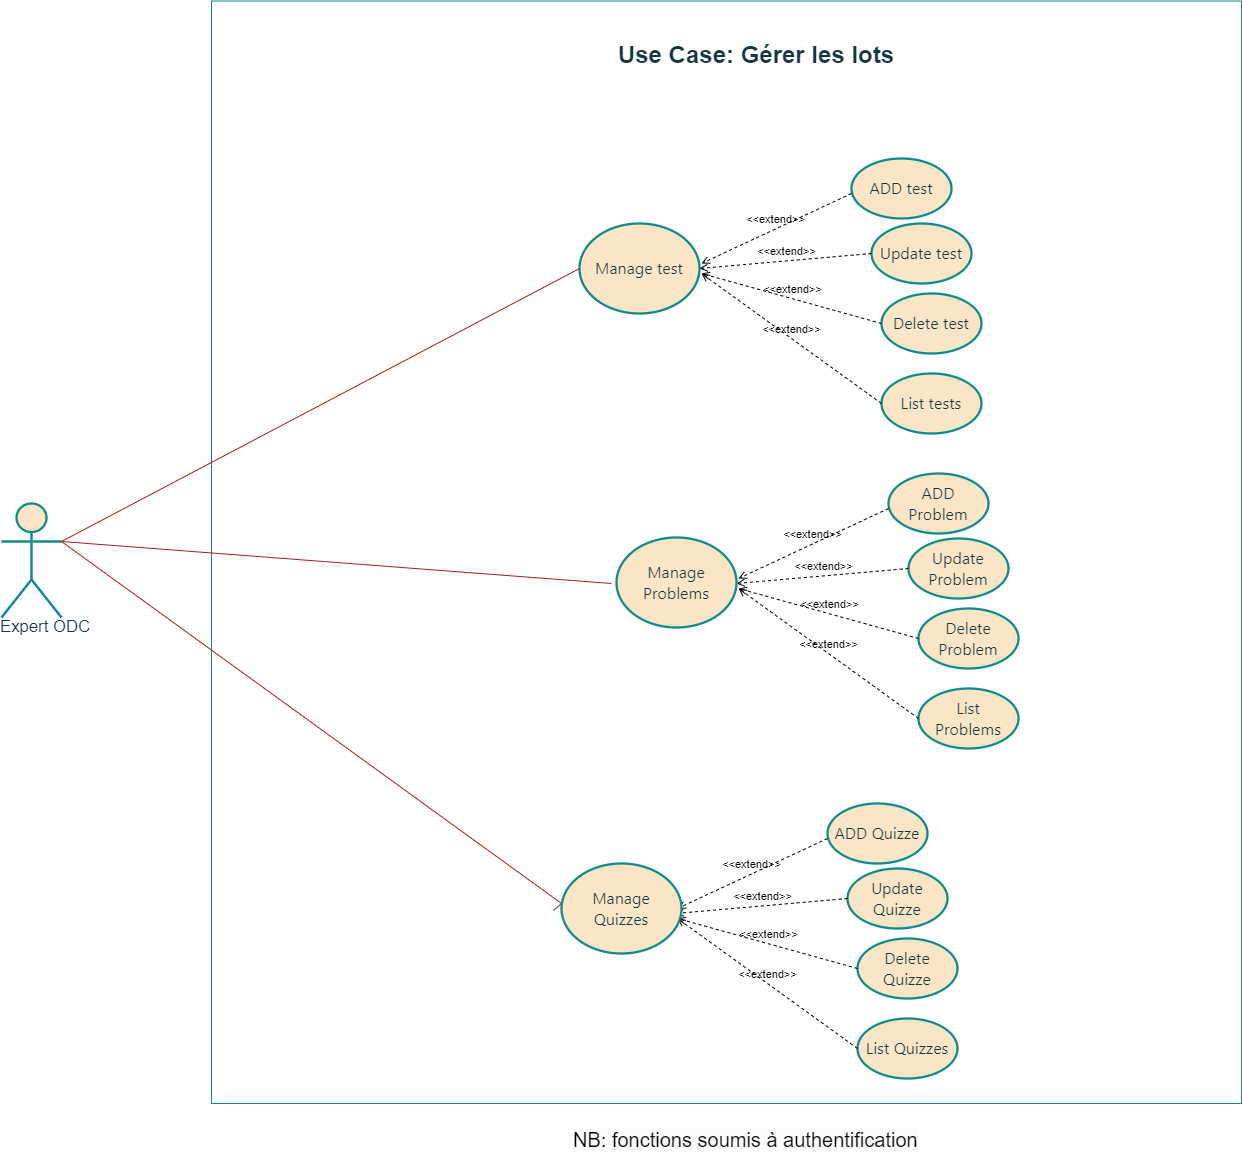
\includegraphics[width=0.8\textwidth]{images/use-case3.png}
    \caption{Use Case Diagram for Sprint 2}
    \label{fig:Use Case Diagram for Sprint 2}
\end{figure}
\subsection{Textual Description of the Use Case "Create a Problem"}

\begin{table}[h]
    \centering
    \begin{tabular}{|c|p{12cm}|}
        \hline
        Use Case & Create a Problem \\
        \hline
        Actor & Expert  \\
        \hline
        Brief Description & The expert wants to create and define a new problem for users to solve. The expert enters the problem name, description, code template, test cases, and solution. The system tests the provided solution against the defined test cases before saving the problem. \\
        \hline
        Pre-condition & The expert is logged into the system and has access to the "Create Problem" interface. \\
        \hline
        Post-condition & The new problem is tested and saved in the system, and is available for users to solve. \\
        \hline
        Main Scenario & \begin{tabular}[c]{@{}l@{}} 
            1. The expert navigates to the "Create" section from the left-side menu. \\
            2. The system displays the "Create Problem" interface. \\
            3. The expert enters the problem name in the "Problem name" field. \\
            4. The expert provides a detailed description in \\the "Problem description" field. \\
            5. The expert writes a code template in the "code template" text area. \\
            6. The expert defines test cases in the "Test Cases" section. \\
            7. The expert writes a sample solution in the "Solution" section. \\
            8. The expert clicks the "Test Problem" button to test the \\problem and solution. \\
            9. The system runs the provided solution against the test cases\\ and displays the results. \\
            10. If the solution passes all test cases, the expert clicks the \\"Create Problem" button to save the problem. \\
            11. The system validates the information and saves \\the problem to the database.
        \end{tabular} \\
        \hline
        Exception Scenario & \begin{tabular}[c]{@{}l@{}} 
            1. Invalid Input: \\
            1.1 If the expert enters invalid or incomplete information, the system \\displays error messages indicating the specific issues. \\
            1.2 The expert corrects the errors and attempts to create the problem again. \\
            2. Test Problem Failure: \\
            2.1 If the provided solution does not pass the test cases, the system displays \\the test results indicating the failures. \\
            2.2 The expert reviews and corrects the solution or test cases and tests \\the problem again.
        \end{tabular} \\
        \hline
        Extension & If the system encounters any issues during validation or database updates, appropriate error messages are displayed, and the expert is prompted to correct the issues. If the system cannot connect to the database, an error message is displayed and the operation is aborted. \\
        \hline
    \end{tabular}
   
    \begin{center}
        \caption{Textual Description of the Use Case "Create a Problem"}
        \label{tab:Textual Description of the Use Case "Create a Problem"}
       
    \end{center}   
\end{table}
 \subsection{the sequence diagram for the use case'Add problem'} 
 \newpage
\begin{figure}[h!]
    \centering*
    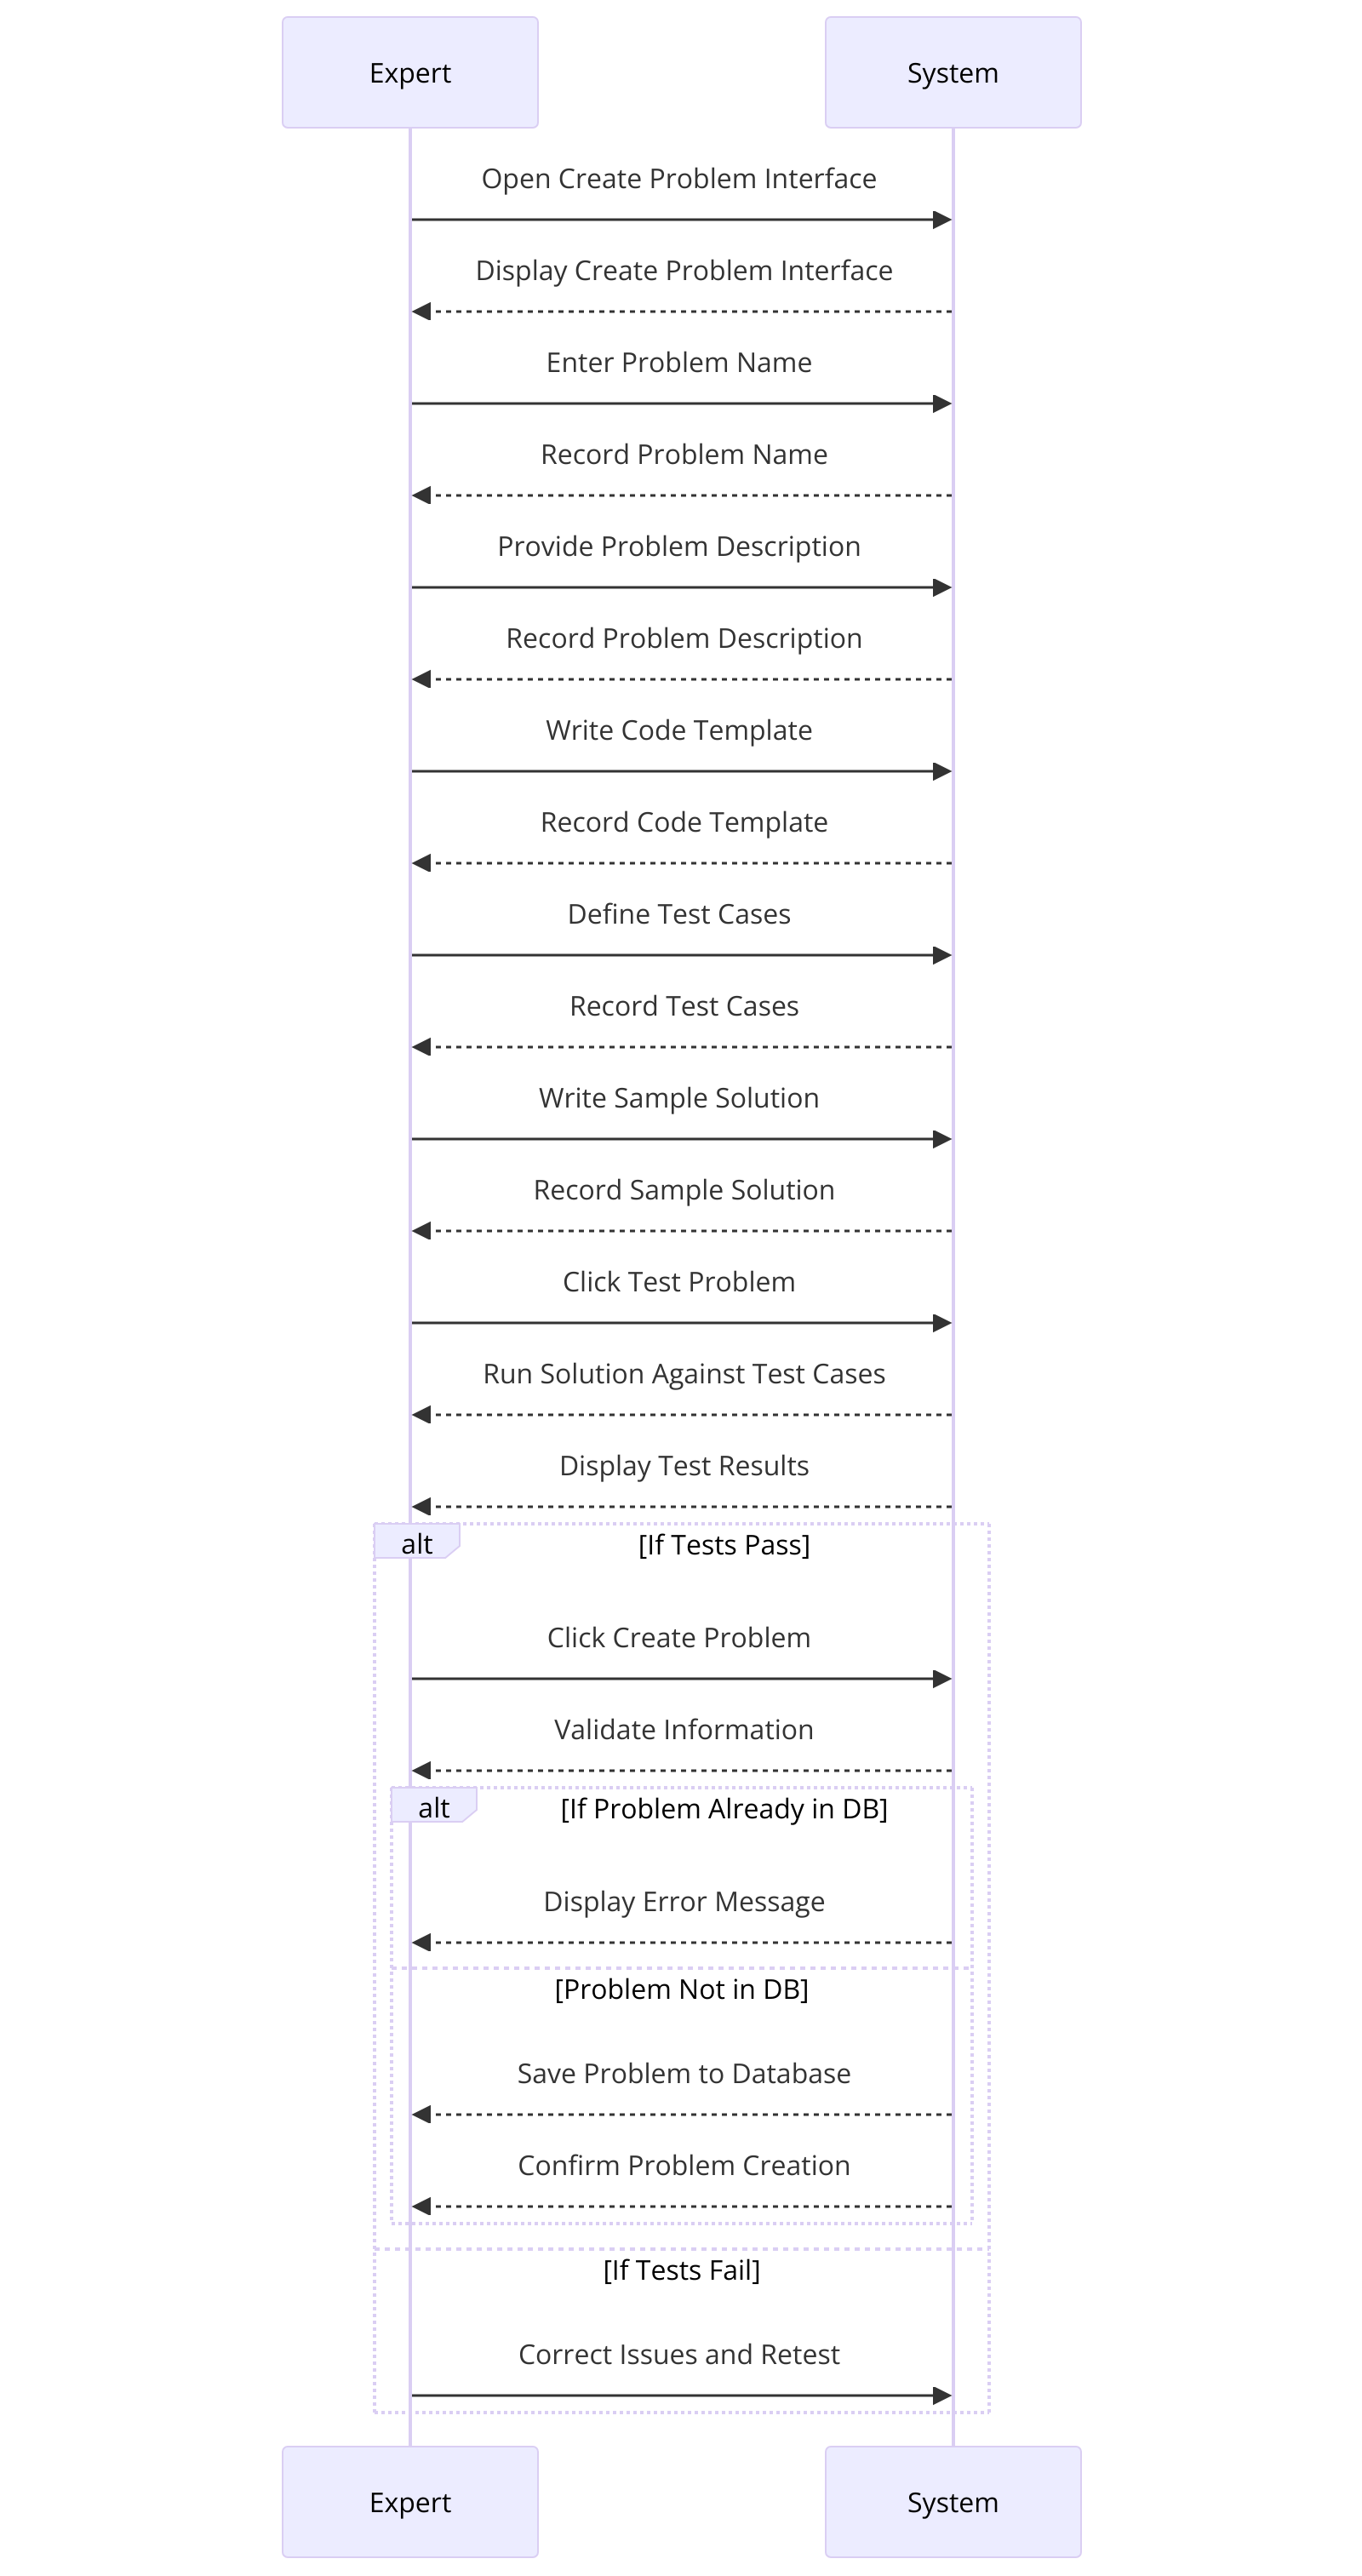
\includegraphics[width=0.8\textwidth]{images/diagram (6).png}
    \caption{the sequence diagram for the use case 'Add problem'}
    \label{fig:the sequence diagram for the use case 'Add problem'}
\end{figure}
